\documentclass[tikz,border=1mm,10pt]{standalone}
%\usepackage[dvipsnames]{xcolor}
\usepackage{pgfplots}
\pgfplotsset{compat=1.5.1}
\begin{document}
	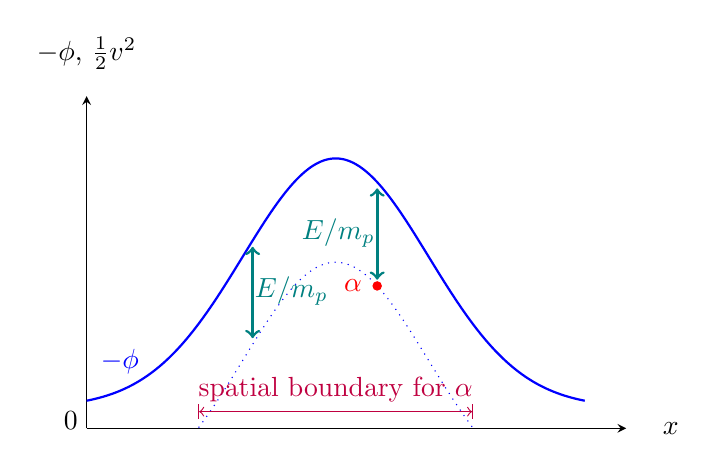
\begin{tikzpicture}[xscale=1,yscale=1,samples=400, transform shape]
	\begin{axis}[
	ticks=none,
	ymin=0,
	ymax=8,
	xmin=-6,
	xmax=7,
	axis x line=bottom,axis y line=left,
	%	axis lines = left,
	xlabel = $x$,
	ylabel = {$- \phi$, $\frac{1}{2} v^2$},
	legend pos=north west,
	every axis x label/.style={
		at={(ticklabel* cs:1.05)},
		anchor=west,
	},
	every axis y label/.style={
		at={(ticklabel* cs:1.05)},
		anchor=south,
	},
	axis equal image
	]
	
	%clump 
	\addplot [
	domain=-6:6, 
	samples=400, 
	color=blue, thick
	]
	{6*exp( (-x^2)/10)+0.5};
%	\addlegendentry{$\phi_B$}

	%dotted
	\addplot [
	domain=-6:6, 
	samples=400, 
	color=blue, dotted
	]
	{6*exp( (-x^2)/10)-2};
		
	% Particles
%	\draw[red,fill] (600,400) circle (.1) node [left = .7mm] {$\alpha$};
	\draw[red,fill] (700,342.902) circle (.1) node [left = .7mm] {$\alpha$};

	% added + 15 pt un lower value and -15 for upper value of y axis for visibility
	\draw[<->, color=teal, line width=1] (700,357.902) -- node [right = -14, above = -3mm] {$E/m_p$} +(0,220);
	\draw[<->, color=teal, line width=1] (400,217.192) -- node [right = 14, above = -3mm] {$E/m_p$} +(0,220);
	\draw[|<->|,color=purple] (600-331.453,40) -- node [anchor=south] {spatial boundary for $\alpha$} (600+331.453,40) ;
	
	%Naming
	\node[thick, blue] at (80,160) {$-\phi$};
	\end{axis};
	\node[] at (-0.2,0.1) {$0$};
	\end{tikzpicture}
\end{document}